% -*- root: main.tex -*-
% @Author: Oscar Esteban
% @Date:   2015-08-12 18:41:16
% @Last Modified by:   Oscar Esteban
% @Last Modified time: 2015-08-14 09:40:31
\documentclass[tikz]{standalone}
\usepackage{graphicx}

\usepackage[T1]{fontenc}
\usepackage{charter}

\def\helveticabold{\fontfamily{phv}\bfseries\selectfont}

\begin{document}
\begin{tikzpicture}
  \node[](fig02a) at (0,5.8)
    {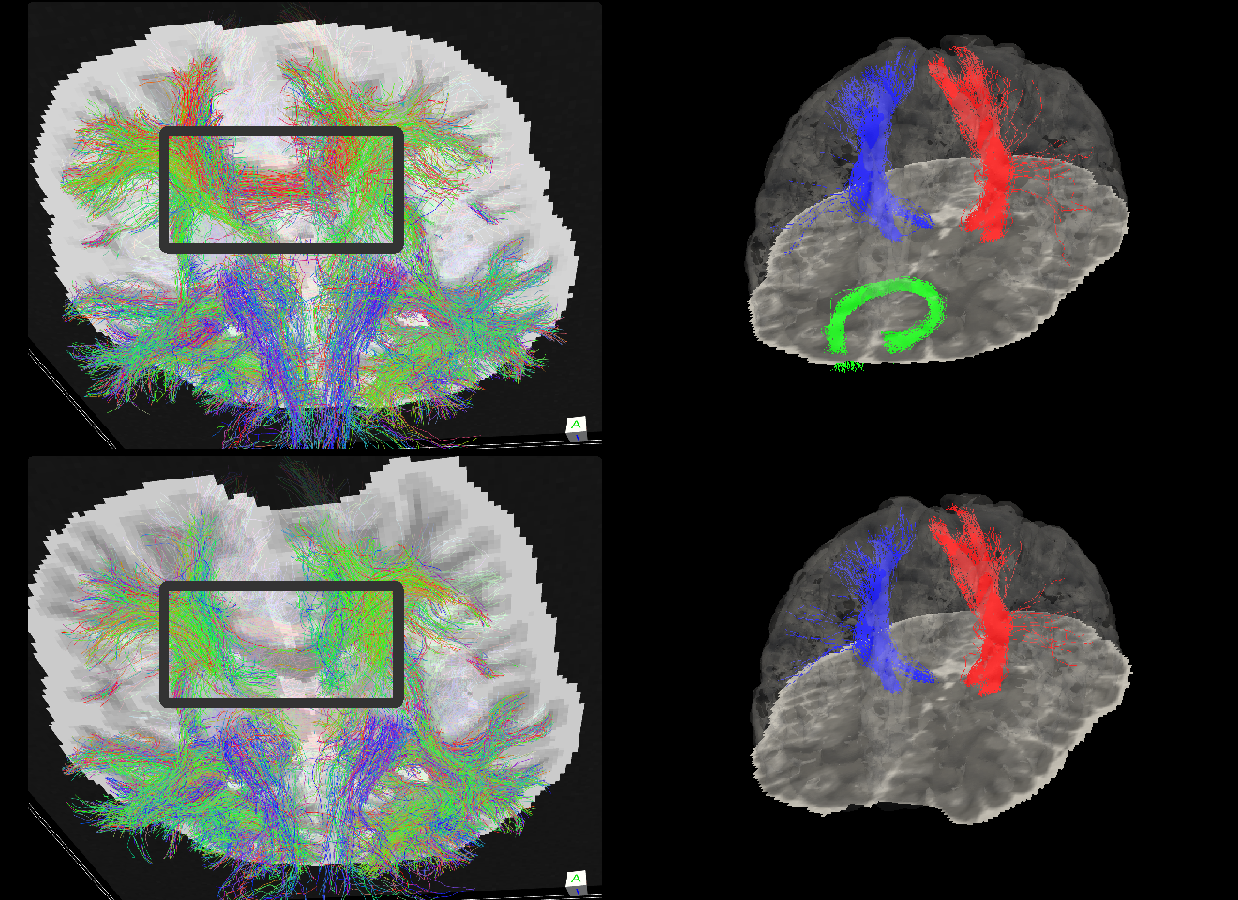
\includegraphics[width=\textwidth]{figures/figure02B}};
  \node[](fig02b) at (0,0)
    {\hspace{1cm}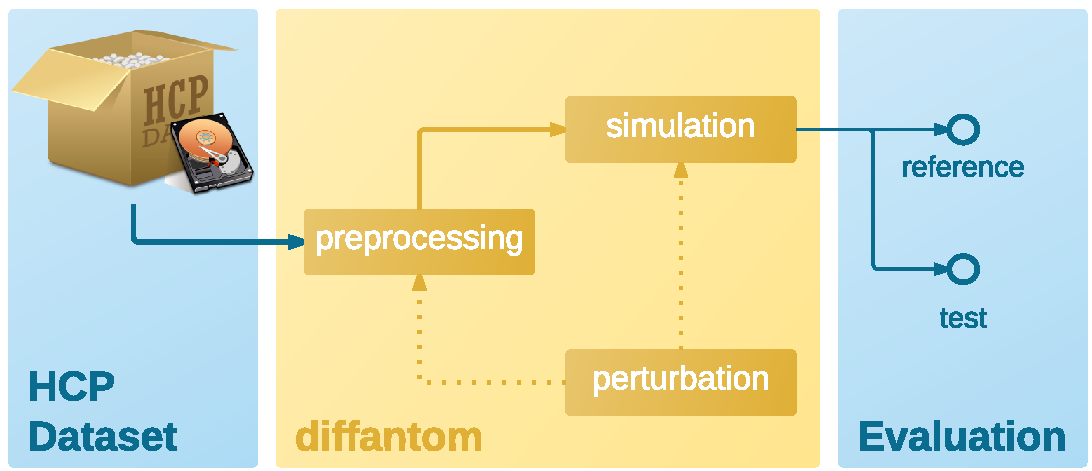
\includegraphics[width=\textwidth]{figures/figure02A}};
  \node[circle, text=white] at (-5.3,7.4) {\helveticabold\fontsize{20}{13}\selectfont{A1}};
  \node[circle, text=black] at (5.3,7.4) {\helveticabold\fontsize{20}{13}\selectfont{A2}};
  \node[circle, text=black] at (-6.0,1.8) {\helveticabold\fontsize{20}{13}\selectfont{B}};
\end{tikzpicture}
\end{document}